\documentclass[11pt, oneside]{article}   	% use "amsart" instead of "article" for AMSLaTeX format
\usepackage{geometry}                		% See geometry.pdf to learn the layout options. There are lots.
\geometry{letterpaper}                   		% ... or a4paper or a5paper or ... 
%\geometry{landscape}                		% Activate for rotated page geometry
%\usepackage[parfill]{parskip}    		% Activate to begin paragraphs with an empty line rather than an indent
\usepackage{graphicx}				% Use pdf, png, jpg, or eps§ with pdflatex; use eps in DVI mode
								% TeX will automatically convert eps --> pdf in pdflatex		
\usepackage{amssymb}

%SetFonts

%SetFonts


\title{ME 459 - HW 8}
\author{Jackson Fox}
\date{Due 11/18}							% Activate to display a given date or no date

\begin{document}
\maketitle
\section*{Task 1}
\subsection*{Plot of Performance}
		\begin{figure} [h]
			\centering
			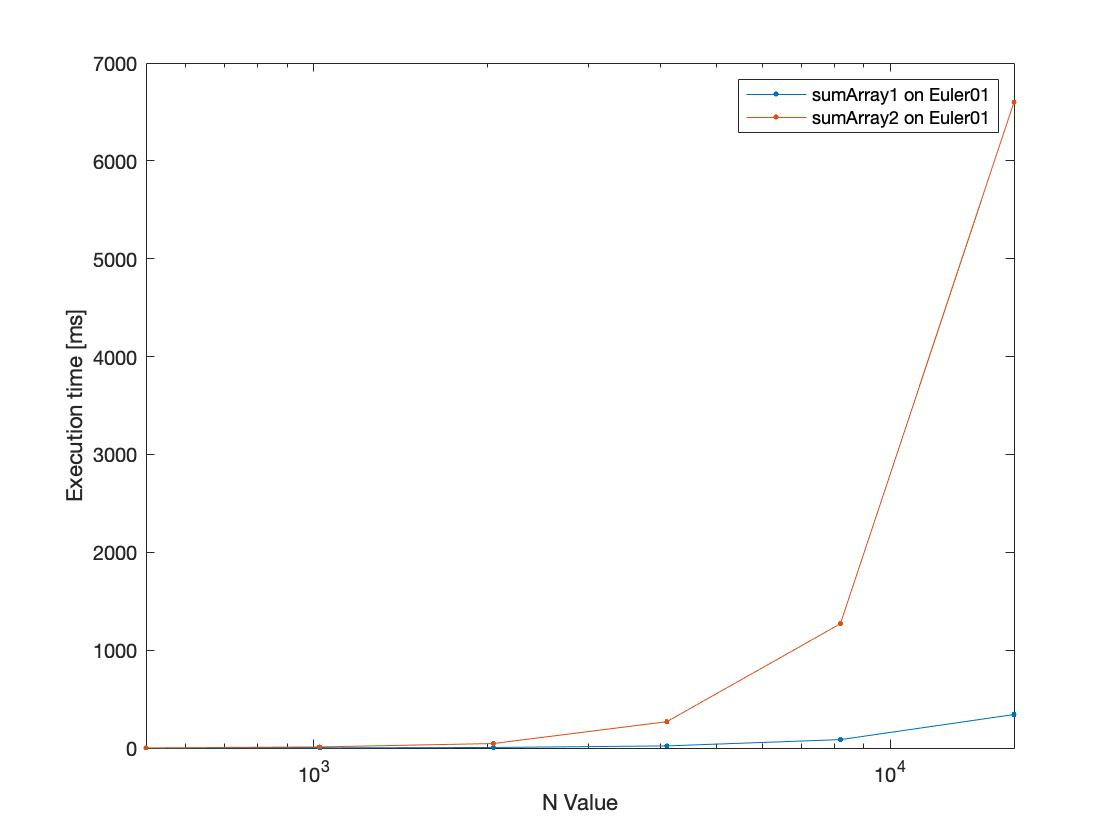
\includegraphics[width=150mm]{Task1.jpg}
			\caption{Plot of performance of sumArray1 and sumArray2 in milliseconds}
		\end{figure}
\subsection*{Part e}
The performance difference is due to the way that the functions parse through the arrays.  In sumArray1, the entries in the array are accessed in row order, which is the same as how the entries are stored in memory.  This means that a substantial number of consecutive entries are stored in the cache at once, minimizing hits to main memory, allowing for quick access.  In sumArray2, the entries are accessed in column order, which is not the same as how they are stored in memory.  This means that it is unlikely that when the program looks for the next entry to add that it's in the cache - to be able to access the next column the program needs to go to main memory which is significantly slower.  As the number of entries in the array increase, the number of hits to the main memory also increases, which causes the dramatic slow down of the sumArray2 vs. sumArray1 with increasing n values.
\section*{Task 2}
\subsection*{Part f}
Of the four implementations, the fastest was mmul3 which took about 1.23 seconds, and the slowest by far was mmul4 which took about 20.13 seconds.  Both mmul1 and mmul2 feel around 9 seconds to complete.  The reason mmul3 is so much more efficient is due to the structure of the B Array.  By utilizing the three for-loop approach and having B column major order, the k index sweeps through both the A and B Arrays row by row, which matches the way that the arrays are stored in memory.  This means that accessing the next element in memory for both arrays can be typically be done in the cache, saving significant time from going to the main memory.  The exact opposite is true in mmul4.  By flipping array A to be in column major order, the k index now sweeps through both array A and B by column.  This is not aligned with how the arrays are stored in memory, and will result in many cache misses when trying to locate subsequent steps.  This requires going to the main memory to find the subsequent steps which is significantly less efficient.
\end{document}  